%!TEX root = etdrtemplate.tex
% +--------------------------------------------------------------------+
% | Sample Chapter 2
% +--------------------------------------------------------------------+

\cleardoublepage

% +--------------------------------------------------------------------+
% | Replace "This is Chapter 2" below with the title of your chapter.
% | LaTeX will automatically number the chapters.
% +--------------------------------------------------------------------+

\chapter{Background}
\label{background}

General overview of all below things?

\section{High-assurance systems}
\label{background:highas}
What software properties and requirements exists to ensure safety.
Medical Devices as High-assurance systems.


\section{SPARK/Ada}
\label{background:spark}
History of Ada: http://www.adahome.com/History/Steelman/intro.htm 
Ada fulfill US DOD requirements.
Rationale of this language. Good for Software Verification etc.
\begin{figure}[ht]%t=top, b=bottom, h=here
    \begin{center}
    	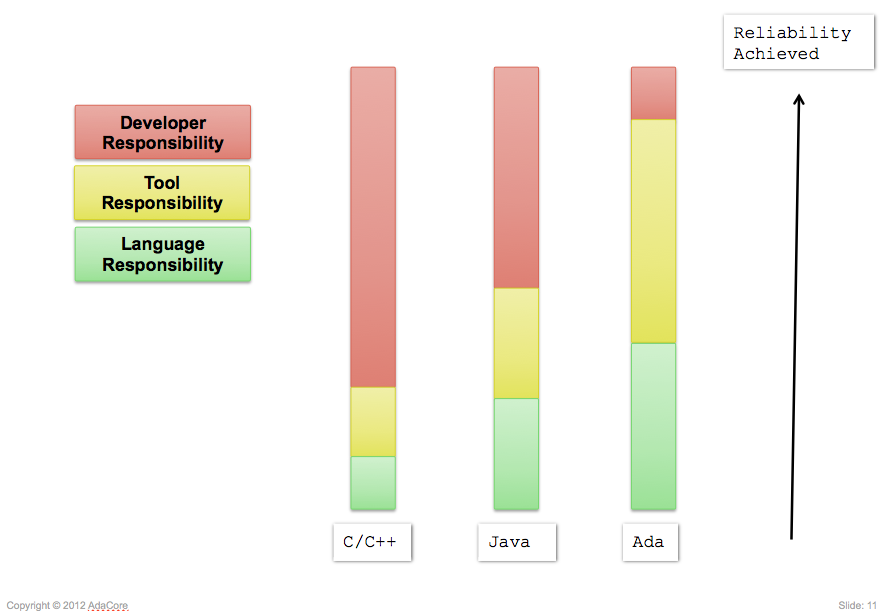
\includegraphics[height=4.5in]{figures/developer_responsibility_in_ada.png}
    	\caption{Developer responsibility in Ada.}
    \end{center}
\end{figure}
%http://www.slideshare.net/AdaCore/ada-2012 (slide 11: dev responsibility)
GNAT Programming Studio. 
Tools for corectness proving.

\subsection{GNAT Programming Studio}
\label{background:spark:gps}
IDE for SPARK/Ada programs development. Includes proving tools. E.g. Sireum Kiasan (developed by SAnToS lab) or GNAT Prove.

\subsection{Sireum Kiasan}
\label{background:spark:sireum}
Overview: symbolic execution, Pilar, Alir\cite{THB}?
Sireum Kiasan\cite{DLR} is a tool, which use symbolic execution for finding possible paths in program.
Plugin for GNAT Programming Studio.
Plugin for Eclipse (but only SPARK 2005).

\subsection{GNAT Prove}
\label{background:spark:gnatprove}
Overview
%http://docs.adacore.com/spark2014-docs/html/ug/gnatprove.html

\subsection{AUnit}
\label{background:spark:aunit}
Overview
AUnit tutorials \cite{AUnitTutorials:Online}
AUnit Cookbook \cite{AUnitCookbook:Online}


\section{AADL}
\label{background:aadl}
Rationale of this language.
“AADL” stands for Architecture Analysis \& Design Language. The aim of the AADL is to allow the description of Distributed Real-Time Embedded (DRE) systems by assembling separately developed blocks. Thus it focuses on the definition of clear block interfaces, and separates the implementations from those interfaces. AADL allows for the description of both software and hardware parts of a system. %http://libre.adacore.com/tools/ocarina/
AADL is a language for Model-Based Engineering\cite{Fei13}.
%https://wiki.sei.cmu.edu/aadl/index.php/The_Story_of_AADL

\subsection{Osate}
\label{background:aadl:osate}
OSATE is a set of plug-ins on top of the open-source Eclipse platform to provide a toolset for front-end processing of AADL models. It is developed mainly by SEI (Software Engineering Institute - CMU). %http://www.aadl.info/aadl/currentsite/tool/osate.html


\section{BLESS}
\label{background:bless}
How it fits into the picture. Why it was developed. Corectness prove in AADL + bahavior, from which we can generate SPARK/Ada code.


\section{Integrated Clinical Environment}
\label{background:ice}
http://santos.cis.ksu.edu/MDCF/doc/ICE-Motivation.pdf
http://santos.cis.ksu.edu/MDCF/doc/MDCF-Tutorial-Overview.pdf


\section{PCA Pump}
\label{background:pcapump}
http://www.santoslab.org/pub/paper/LarsonEtAl13-PCA-Requirements-SEHC-preprint.pdf


\section{AADL/BLESS to SPARK/Ada code generation(maybe translation is better word?)}
\label{background:codegen}
The ultimate goal of long term research, this thesis is part of.
AADLto Ada
BLESS to SPARK contracts + (eventually) behavior

\subsection{Ocarina}
\label{background:codegen:ocarina}
Overview: AADL->Ada on PolyOrb, support for other languages?

Ocarina generate code from an AADL architecture model to an Ada application running on top of PolyORB framework. In this context, PolyORB acts as both the distribution middleware and execution runtime on all targets supported by PolyORB.
It generate Ada 2005 and C code.


\subsection{Ramses}
\label{background:codegen:ramses}
Overview. Not sure if it is useful at any point here?